%*************************************
% บทที่ 4
%*************************************
\chapterTitle{4}{ผลการดำเนินงาน}

\hspace*{1.5em}
ในการพัฒนาระบบแพลตฟอร์มคลาวด์เพื่อสนับสนุนกิจกรรมการเรียนการสอนและงานวิชาการ ได้ดำเนินการออกแบบและพัฒนาระบบที่ประกอบด้วย 3 ส่วนหลัก คือ ส่วนติดต่อผู้ใช้ (Frontend) ส่วนบริการ API (API Service) และส่วนจัดการเครื่องเสมือน (VM Operations Service) 
พร้อมทั้งระบบฐานข้อมูล ระบบคิวข้อความ และระบบติดตามการทำงาน ในส่วนของผลการดำเนินงานที่ได้จะประกอบด้วยโครงสร้างโปรเจกต์ การจัดการไฟล์และโฟลเดอร์ การกำหนดค่าระบบ และการจัดการแพ็กเกจต่าง ๆ 
ทั้งนี้ ระบบที่พัฒนาขึ้นได้ถูกออกแบบให้รองรับการทำงานแบบ Microservices Architecture เพื่อความยืดหยุ่นในการขยายระบบและการบำรุงรักษา โดยใช้เทคโนโลยีสมัยใหม่ที่เหมาะสมกับการใช้งานในสภาพแวดล้อมการศึกษา
\section{โครงสร้างโปรเจกต์หลัก}
\hspace*{1.5em}
จากการออกแบบและพัฒนาระบบแพลตฟอร์มคลาวด์เพื่อสนับสนุนกิจกรรมการเรียนการสอนและงานวิชาการ ระบบประกอบไปด้วย 3 โฟลเดอร์หลัก ได้แก่ 

\subsection{โฟลเดอร์ Apps}
\hspace*{1.5em}
โฟลเดอร์ \textbf{Apps} เป็นที่เก็บแอปพลิเคชันหลักทั้งหมดของระบบ ซึ่งประกอบด้วย 3 บริการหลัก คือ \textbf{Midori}, \textbf{Momoi}, และ \textbf{Yuzu} ที่ทำงานร่วมกันในรูปแบบ Microservices Architecture 
\begin{mycustomenum2}
  \item \textbf{Midori} - ส่วนติดต่อผู้ใช้ (Frontend) ที่พัฒนาด้วย Next.js
  \item \textbf{Momoi} - บริการ API หลัก (API Service) ที่พัฒนาด้วย Elysia.js  
  \item \textbf{Yuzu} - บริการจัดการเครื่องเสมือน (VM Operations Service)
\end{mycustomenum2}
\hspace*{1.5em}
แต่ละบริการในโฟลเดอร์ \textbf{Apps} มีโครงสร้างและหน้าที่เฉพาะตัว โดยการแยกเป็นบริการย่อยจะช่วยให้ระบบมีความยืดหยุ่นในการพัฒนา การทดสอบ และการบำรุงรักษา

\subsection{โฟลเดอร์ Packages}
\hspace*{1.5em}
โฟลเดอร์ \textbf{Packages} ใช้สำหรับเก็บแพ็กเกจและไลบรารีที่ใช้ร่วมกันระหว่างบริการต่าง ๆ ในระบบ ภายในโฟลเดอร์นี้จะเก็บโค้ดที่สามารถนำไปใช้ซ้ำได้ (Reusable Code) เพื่อลดการเขียนโค้ดซ้ำซ้อน 
ตัวอย่างแพ็กเกจที่เก็บ ได้แก่
\begin{mycustomenum2}
  \item \textbf{Auth} - จัดการระบบยืนยันตัวตนและการให้สิทธิ์
  \item \textbf{Database} - จัดการฐานข้อมูลและ ORM Models
  \item \textbf{Utils} - ฟังก์ชันและเครื่องมือที่ใช้ร่วมกัน
\end{mycustomenum2}
\hspace*{1.5em}
การจัดระเบียบแพ็กเกจในโฟลเดอร์ \textbf{Packages} จะช่วยให้การจัดการโค้ดเป็นระเบียบ สะดวกต่อการบำรุงรักษา และสามารถนำไปใช้ในโปรเจกต์อื่น ๆ ได้ง่าย

\subsection{โฟลเดอร์ Config}
\hspace*{1.5em}
โฟลเดอร์ \textbf{Config} ใช้สำหรับเก็บไฟล์การกำหนดค่าต่าง ๆ ของระบบ เช่น การกำหนดค่าบริการ Infrastructure การตั้งค่า Monitoring และการกำหนดค่า Cloud Scripts ที่จำเป็นสำหรับการทำงานของระบบ โดยการแยกไฟล์การกำหนดค่าออกมาเป็นโฟลเดอร์แยกจะช่วยให้ง่ายต่อการจัดการและแก้ไขการตั้งค่าของระบบ โดยไม่ต้องไปแก้ไขโค้ดหลักของแอปพลิเคชัน

\section{โครงสร้างแอปพลิเคชันและบริการ}
\subsection{ส่วนประกอบหลักของระบบ}
\hspace*{1.5em}
นอกจากโฟลเดอร์ทั้งสามที่กล่าวมาแล้ว ในโครงสร้างโปรเจกต์ยังมีไฟล์และโฟลเดอร์สำคัญอื่น ๆ อีกหลายส่วน ได้แก่ ไฟล์ \textbf{package.json} ซึ่งเป็นไฟล์หลักที่ใช้ในการจัดการ Monorepo และกำหนด Workspaces สำหรับแต่ละแอปพลิเคชันและแพ็กเกจ 
ไฟล์นี้จะทำหน้าที่กำหนดการพึ่งพา (Dependencies) ระหว่างแพ็กเกจต่าง ๆ รวมถึงการตั้งค่า TypeScript และ Bun Runtime ที่ใช้ในการพัฒนาและรันแอปพลิเคชัน พร้อมทั้งจัดการ Scripts สำหรับการ Build, Test, และ Deploy ระบบ ทำให้ผู้พัฒนาสามารถจัดการโปรเจกต์ขนาดใหญ่ได้อย่างเป็นระบบและมีประสิทธิภาพ

\subsection{โครงสร้างระบบทั้งหมด}
\hspace*{1.5em}
ภาพที่ \ref{fig4:ProjectStructure} แสดงโครงสร้างโปรเจกต์ทั้งหมดของระบบแพลตฟอร์มคลาวด์เพื่อสนับสนุนกิจกรรมการเรียนการสอนและงานวิชาการ จะเห็นว่ามีการจัดระเบียบไฟล์และโฟลเดอร์อย่างเป็นระบบ เพื่อความสะดวกในการพัฒนาและบำรุงรักษา โดยโครงสร้างประกอบด้วยโฟลเดอร์หลัก 3 โฟลเดอร์ ได้แก่ Apps, Packages และ Config ซึ่งทำหน้าที่จัดการแอปพลิเคชัน แพ็กเกจร่วม และการกำหนดค่าตามลำดับ อีกทั้งยังมีโฟลเดอร์เสริมอื่น ๆ เช่น Docker และ Docs ดังที่กล่าวไว้ข้างต้น

\hspace*{1.5em}
นอกจากนี้ยังประกอบด้วยไฟล์สำคัญอีกหลายไฟล์ ได้แก่
\begin{mycustomitem}
    \item docker-compose.yaml สำหรับการจัดการ Infrastructure Services
    \item tsconfig.json สำหรับการกำหนดค่า TypeScript ทั้งโปรเจกต์
    \item bun.lock สำหรับล็อกเวอร์ชันของแพ็กเกจที่ใช้
    \item .env.example สำหรับตัวอย่างการตั้งค่าตัวแปรสภาพแวดล้อม
    \item setup.sh และ setup.ps1 สำหรับสคริปต์การติดตั้งเริ่มต้น
    \item ไฟล์เอกสารต่าง ๆ เช่น README.md และ TODO.md
\end{mycustomitem}
\hspace*{1.5em}
การแบ่งโครงสร้างเป็นส่วนย่อยเช่นนี้ช่วยให้การจัดการโปรเจกต์มีความเป็นระเบียบ และง่ายต่อการทำงานร่วมกันเป็นทีม เมื่อต้องการแก้ไขหรือเพิ่มฟีเจอร์ในบริการใดบริการหนึ่งก็สามารถเข้าไปทำงานได้โดยตรงในโฟลเดอร์นั้น ๆ โดยไม่กระทบกับส่วนอื่น ๆ ของระบบ

\begin{figure}[htbp]
\centering
\adjustbox{frame, width=0.8\textwidth}{
    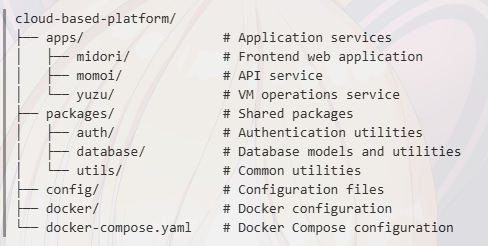
\includegraphics[width=0.8\textwidth]{Image/web/project_structure.png}
}
\caption{\fontSixTeen{โครงสร้างโปรเจกต์ทั้งหมด}}
\label{fig4:ProjectStructure}
\end{figure}

\hspace*{1.5em}
การจัดโครงสร้างโปรเจกต์ในลักษณะ Monorepo นี้ไม่เพียงแต่ช่วยให้โปรเจกต์เป็นระเบียบ แต่ยังช่วยลดความซับซ้อนในการจัดการ Dependencies ระหว่างแพ็กเกจ ทำให้การพัฒนาและการ Deploy เป็นทีมง่ายขึ้น และสามารถแชร์โค้ดระหว่างบริการต่าง ๆ ได้อย่างมีประสิทธิภาพ

\section{สถาปัตยกรรมระบบและเทคโนโลยี}
\subsection{การออกแบบสถาปัตยกรรมแบบ Microservices}
\hspace*{1.5em}
ระบบแพลตฟอร์มคลาวด์ที่พัฒนาขึ้นใช้สถาปัตยกรรมแบบ Microservices ซึ่งประกอบด้วยบริการหลัก 3 ตัว ที่ทำงานอิสระแต่สื่อสารกันผ่าน API และ Message Queue โดยแต่ละบริการมีหน้าที่และความรับผิดชอบที่แตกต่างกัน เพื่อให้ระบบมีความยืดหยุ่นและสามารถขยายตัวได้ง่าย

\hspace*{1.5em}
ภาพที่ \ref{fig4:SystemArchitecture} แสดงสถาปัตยกรรมระบบโดยรวม โดยมี \textbf{Midori} เป็นส่วนติดต่อผู้ใช้ที่พัฒนาด้วย Next.js และ Material UI \textbf{Momoi} เป็นบริการ API หลักที่จัดการการยืนยันตัวตน การจัดการผู้ใช้ และการเชื่อมต่อกับฐานข้อมูล และ \textbf{Yuzu} เป็นบริการจัดการเครื่องเสมือนที่เชื่อมต่อกับ Proxmox VE ผ่าน RabbitMQ

\begin{figure}[htbp]
\centering
\adjustbox{frame, width=0.9\textwidth}{
    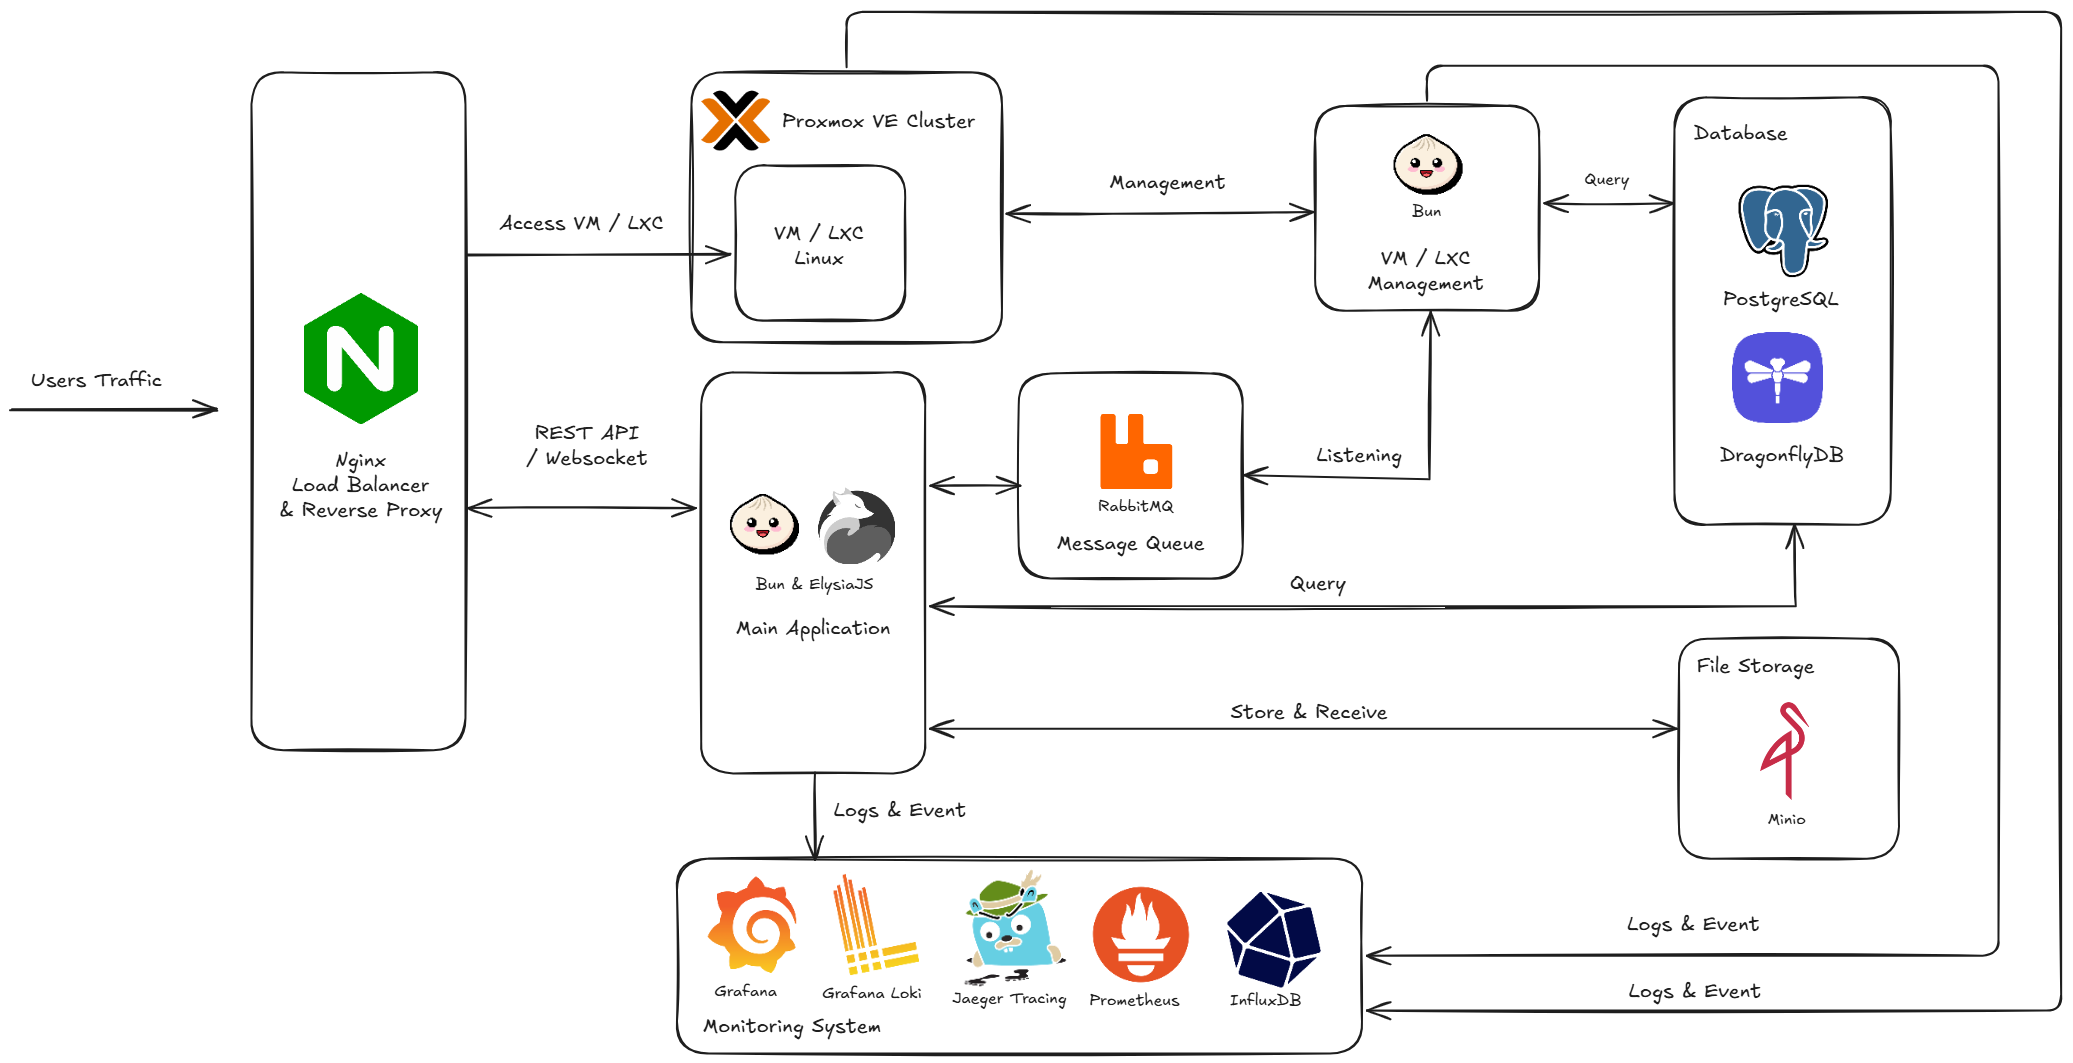
\includegraphics[width=0.9\textwidth]{Image/web/system_architecture.png}
}
\caption{\fontSixTeen{สถาปัตยกรรมระบบโดยรวม}}
\label{fig4:SystemArchitecture}
\end{figure}

\subsection{เทคโนโลยีที่ใช้ในการพัฒนา}
\hspace*{1.5em}
ในการพัฒนาระบบแพลตฟอร์มคลาวด์นี้ ได้เลือกใช้เทคโนโลยีที่ทันสมัยและเหมาะสมกับการใช้งานในสภาพแวดล้อมการศึกษา โดยเทคโนโลยีหลักที่ใช้ประกอบด้วย
\begin{mycustomitem}
    \item \textbf{Bun Runtime} - JavaScript/TypeScript Runtime ที่มีประสิทธิภาพสูง
    \item \textbf{Next.js} - React Framework สำหรับการพัฒนา Frontend
    \item \textbf{Elysia.js} - Web Framework สำหรับการพัฒนา API
    \item \textbf{PostgreSQL} - ระบบจัดการฐานข้อมูลเชิงสัมพันธ์
    \item \textbf{Prisma ORM} - Object-Relational Mapping สำหรับการจัดการฐานข้อมูล
    \item \textbf{RabbitMQ} - Message Queue สำหรับการสื่อสารระหว่างบริการ
    \item \textbf{Docker} - Container Platform สำหรับการ Deploy และการจัดการ Infrastructure
\end{mycustomitem}

\hspace*{1.5em}
การเลือกใช้เทคโนโลยีเหล่านี้มีเหตุผลสำคัญ คือ ความเสถียร ประสิทธิภาพ และการรองรับการขยายระบบในอนาคต รวมถึงการมี Community ที่ใหญ่และเอกสารประกอบที่ครบถ้วน ทำให้การพัฒนาและบำรุงรักษาระบบเป็นไปอย่างราบรื่น

\section{เอกสารประกอบการใช้งาน API และส่วนติดต่อผู้ใช้}
\subsection{เอกสาร API Documentation}
\hspace*{1.5em}
ระบบแพลตฟอร์มคลาวด์ได้จัดทำเอกสาร API Documentation อย่างครบถ้วนโดยใช้ OpenAPI Specification (Swagger) เพื่อให้ผู้พัฒนาและผู้ใช้งานสามารถเข้าใจและใช้งาน API ได้อย่างง่ายดาย เอกสารนี้ประกอบด้วยรายละเอียดของ Endpoints ต่าง ๆ พารามิเตอร์ที่ต้องการ รูปแบบข้อมูลที่ส่งและรับ รวมทั้งตัวอย่างการใช้งานที่ชัดเจน

\hspace*{1.5em}
ภาพที่ \ref{fig4:APIDocumentation} แสดงหน้าเอกสาร API Documentation ที่สร้างขึ้นโดยอัตโนมัติจากโค้ด TypeScript ผ่าน Elysia.js และ OpenAPI Plugin ซึ่งมีการจัดหมวดหมู่ API เป็นกลุ่มต่าง ๆ ดังนี้

\begin{mycustomitem}
    \item \textbf{Public API} - สำหรับการใช้งานทั่วไปที่ไม่ต้องมีการยืนยันตัวตน
    \item \textbf{Authentication API} - สำหรับการล็อกอิน ล็อกเอาต์ และการจัดการเซสชัน
    \item \textbf{Student API} - สำหรับนักศึกษาในการจัดการเครื่องเสมือนส่วนตัว
    \item \textbf{Staff API} - สำหรับอาจารย์และเจ้าหน้าที่ในการจัดการระบบ
    \item \textbf{Admin API} - สำหรับผู้ดูแลระบบในการจัดการผู้ใช้และทรัพยากร
\end{mycustomitem}

\begin{figure}[htbp]
\centering
\adjustbox{frame, width=0.9\textwidth}{
    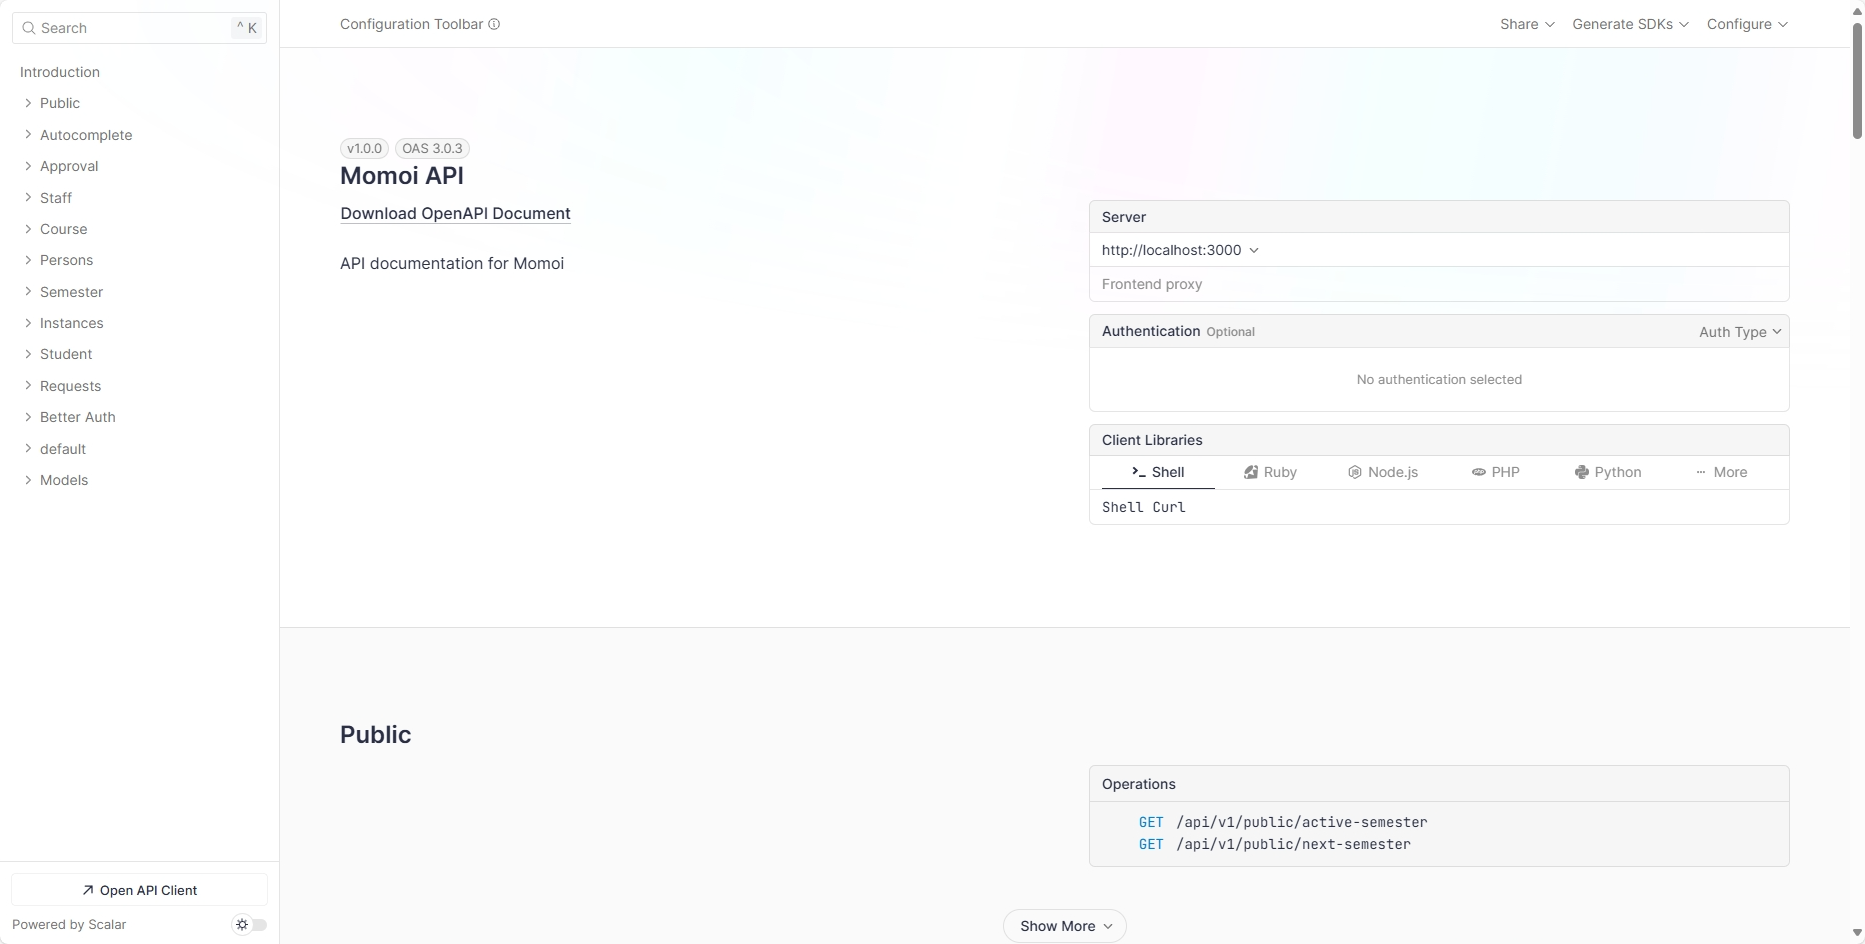
\includegraphics[width=0.9\textwidth]{Image/web/api_documentation.png}
}
\caption{\fontSixTeen{หน้าเอกสาร API Documentation}}
\label{fig4:APIDocumentation}
\end{figure}

\hspace*{1.5em}
เอกสาร API นี้มีการอัปเดตอัตโนมัติเมื่อมีการเปลี่ยนแปลงโค้ด และสามารถทดสอบ API ได้โดยตรงผ่านหน้าเว็บ ทำให้ผู้พัฒนาสามารถทำความเข้าใจและใช้งาน API ได้อย่างรวดเร็วและถูกต้อง

\subsection{ส่วนติดต่อผู้ใช้ (User Interface)}
\hspace*{1.5em}
ส่วนติดต่อผู้ใช้ของระบบได้รับการออกแบบให้ใช้งานง่าย สวยงาม และตอบสนองได้ดีบนอุปกรณ์ต่าง ๆ โดยใช้ Material UI และ Tailwind CSS ในการจัดรูปแบบ ระบบประกอบด้วยหน้าหลักต่าง ๆ ที่มีการจัดระเบียบข้อมูลและฟังก์ชันการทำงานอย่างชัดเจน

\hspace*{1.5em}
ภาพที่ \ref{fig4:LandingPage} แสดงหน้าแรกของระบบ (Landing Page) ที่ออกแบบให้ดึงดูดความสนใจและสื่อสารจุดประสงค์ของระบบได้ชัดเจน โดยมีการนำเสนอฟีเจอร์หลักของระบบ ข้อมูลการติดต่อ และลิงก์สำหรับการล็อกอินเข้าสู่ระบบ

\begin{figure}[htbp]
\centering
\adjustbox{frame, width=0.9\textwidth}{
    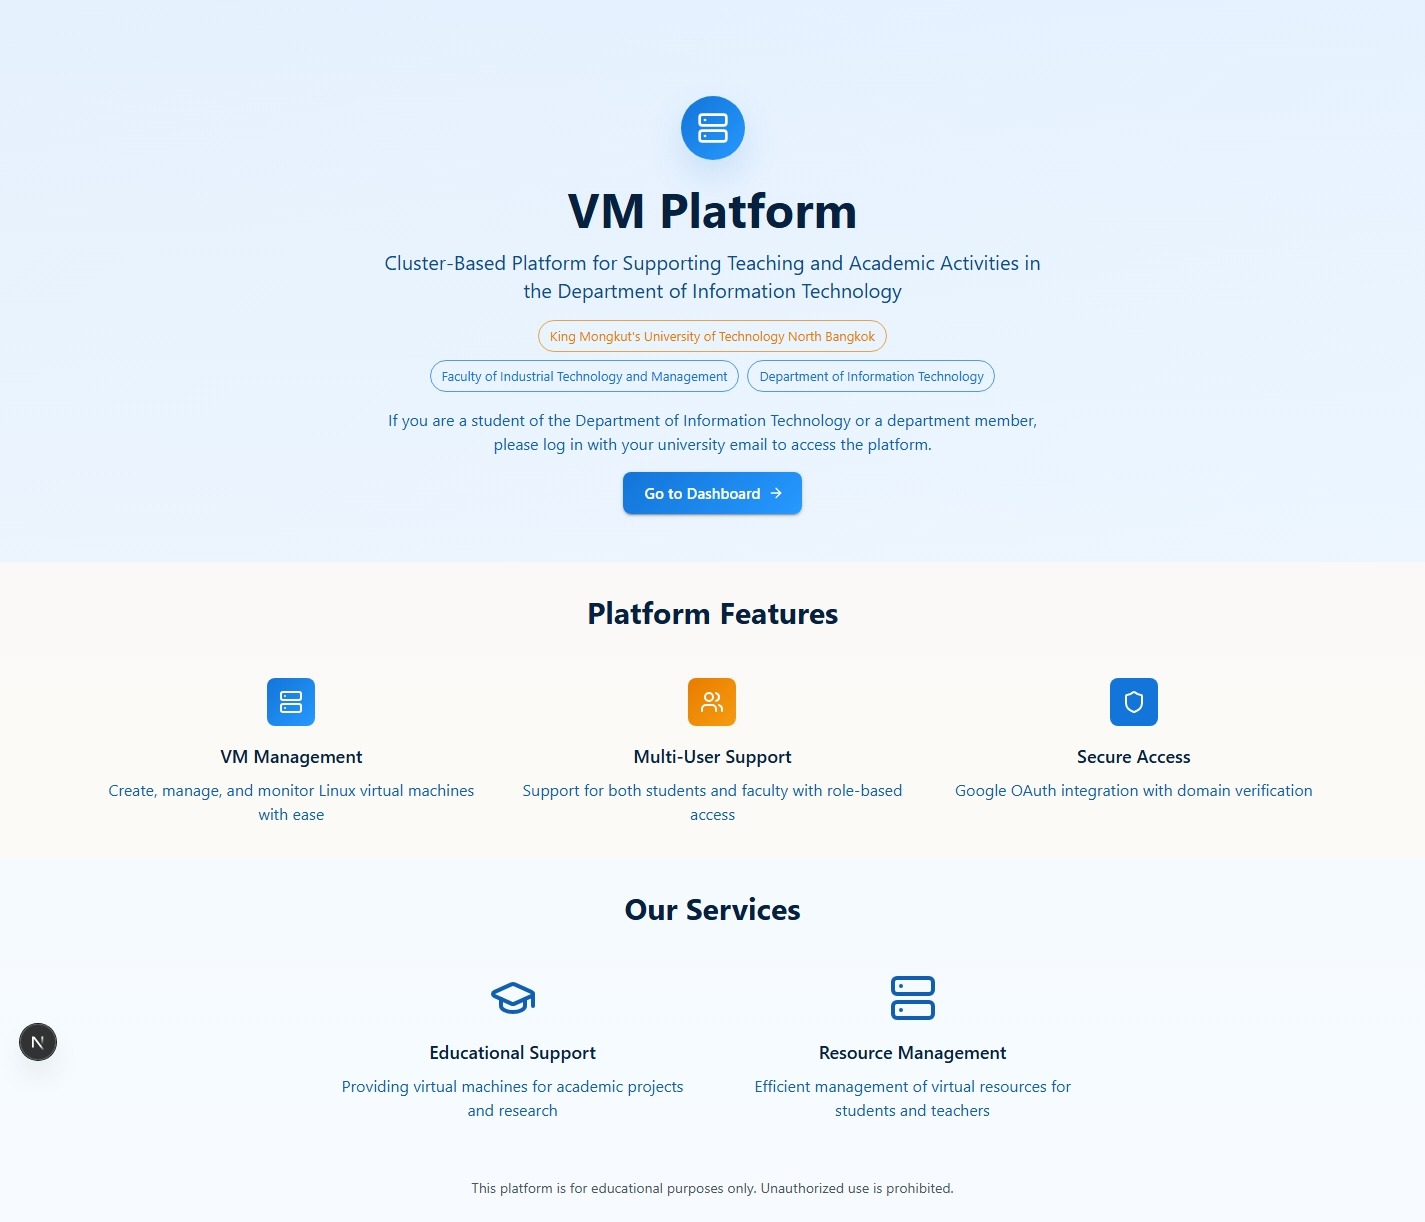
\includegraphics[width=0.9\textwidth]{Image/web/landing_page.jpeg}
}
\caption{\fontSixTeen{หน้าแรกของระบบ (Landing Page)}}
\label{fig4:LandingPage}
\end{figure}

\subsection{Dashboard และระบบจัดการ}
\hspace*{1.5em}
หลังจากที่ผู้ใช้ล็อกอินเข้าสู่ระบบแล้ว ผู้ใช้จะเข้าสู่หน้า Dashboard ที่แสดงข้อมูลสำคัญและฟังก์ชันการทำงานต่าง ๆ ตามบทบาทของผู้ใช้ โดย Dashboard ได้รับการออกแบบให้แสดงข้อมูลอย่างเป็นระบบและเข้าใจง่าย พร้อมทั้งมีการใช้งานที่สะดวกและรวดเร็ว

\hspace*{1.5em}
ส่วนติดต่อผู้ใช้ที่พัฒนาขึ้นมีลักษณะสำคัญดังนี้
\begin{mycustomitem}
    \item \textbf{Responsive Design} - รองรับการแสดงผลบนหน้าจอขนาดต่าง ๆ
    \item \textbf{Intuitive Navigation} - การนำทางที่เข้าใจง่ายและสอดคล้องกับมาตรฐาน UX
    \item \textbf{Real-time Updates} - การอัปเดตข้อมูลแบบเรียลไทม์
    \item \textbf{Accessibility} - การออกแบบที่คำนึงถึงผู้ใช้ที่มีความต้องการพิเศษ
    \item \textbf{Theme Support} - รองรับการเปลี่ยนธีมสีตามความต้องการ
\end{mycustomitem}

\hspace*{1.5em}
การออกแบบส่วนติดต่อผู้ใช้ได้คำนึงถึงประสบการณ์ผู้ใช้ (User Experience) เป็นหลัก โดยมุ่งเน้นให้ผู้ใช้สามารถทำงานได้อย่างมีประสิทธิภาพและลดข้อผิดพลาดในการใช้งาน ทั้งนี้ระบบยังมีการจัดการข้อผิดพลาดและการแจ้งเตือนที่ชัดเจน เพื่อให้ผู้ใช้สามารถแก้ไขปัญหาได้อย่างรวดเร็ว

\section{ตัวอย่างการใช้งานระบบตามบทบาทผู้ใช้}
\subsection{Dashboard สำหรับนักศึกษา}
\hspace*{1.5em}
ระบบได้จัดทำ Dashboard เฉพาะสำหรับนักศึกษา เพื่อให้สามารถจัดการเครื่องเสมือนส่วนตัวและติดตามการใช้งานทรัพยากรได้อย่างง่ายดาย ภาพที่ \ref{fig4:StudentDashboard} แสดง Dashboard หลักของนักศึกษาที่ประกอบด้วยข้อมูลสรุปการใช้งาน สถานะเครื่องเสมือน และฟังก์ชันการจัดการที่สำคัญ

\begin{figure}[htbp]
\centering
\adjustbox{frame, width=0.9\textwidth}{
    
\includegraphics[width=0.9\textwidth]{Image/web/dashboard/student/dashboard.jpeg}
}
\caption{\fontSixTeen{Dashboard หลักสำหรับนักศึกษา}}
\label{fig4:StudentDashboard}
\end{figure}

\hspace*{1.5em}
นักศึกษาสามารถดูรายการเครื่องเสมือนทั้งหมดที่ตนเองมีสิทธิ์เข้าถึง พร้อมทั้งสถานะการทำงาน การใช้ทรัพยากร และการจัดการพื้นฐาน ดังแสดงในภาพที่ \ref{fig4:StudentInstances} ซึ่งนำเสนอรายละเอียดของแต่ละ Instance อย่างชัดเจน

\begin{figure}[htbp]
\centering
\adjustbox{frame, width=0.9\textwidth}{
    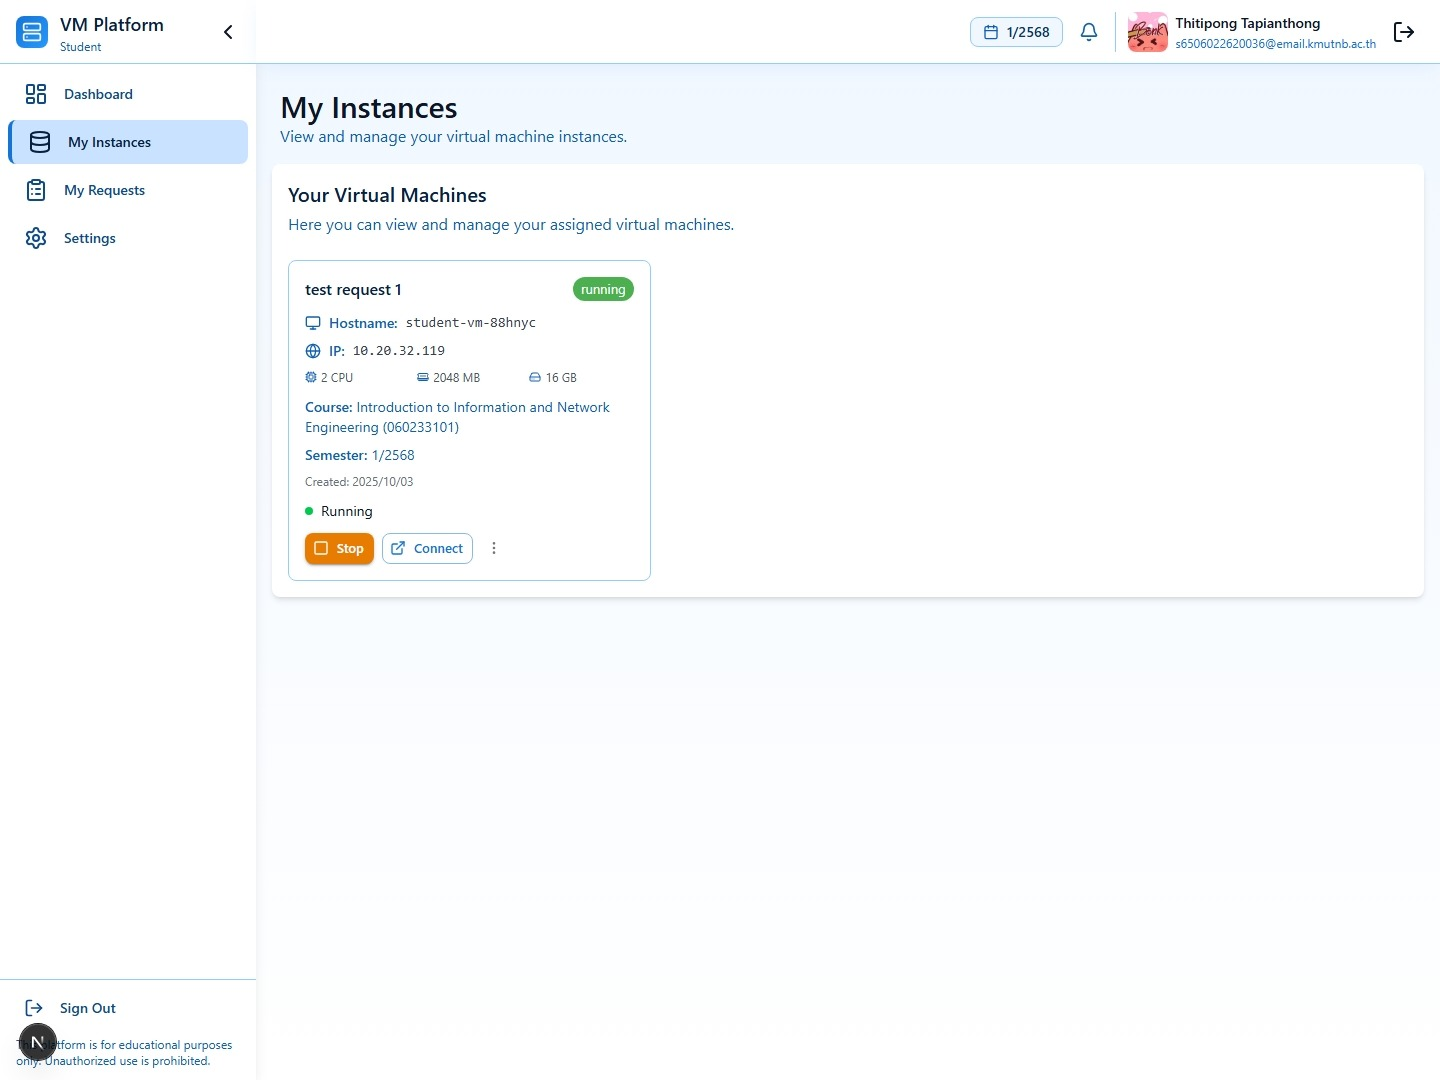
\includegraphics[width=0.9\textwidth]{Image/web/dashboard/student/instances.jpeg}
}
\caption{\fontSixTeen{หน้าจัดการ VM Instances สำหรับนักศึกษา}}
\label{fig4:StudentInstances}
\end{figure}

\subsection{Dashboard สำหรับอาจารย์และเจ้าหน้าที่}
\hspace*{1.5em}
สำหรับอาจารย์และเจ้าหน้าที่ ระบบได้จัดเตรียม Dashboard ที่มีฟังก์ชันการจัดการขั้นสูงมากขึ้น รวมถึงการอนุมัติคำขอ การจัดการหลักสูตร และการตรวจสอบการใช้งานของนักศึกษา ภาพที่ \ref{fig4:StaffDashboard} แสดง Dashboard หลักสำหรับเจ้าหน้าที่ที่มีข้อมูลสถิติและการควบคุมระบบ

\begin{figure}[htbp]
\centering
\adjustbox{frame, width=0.9\textwidth}{
    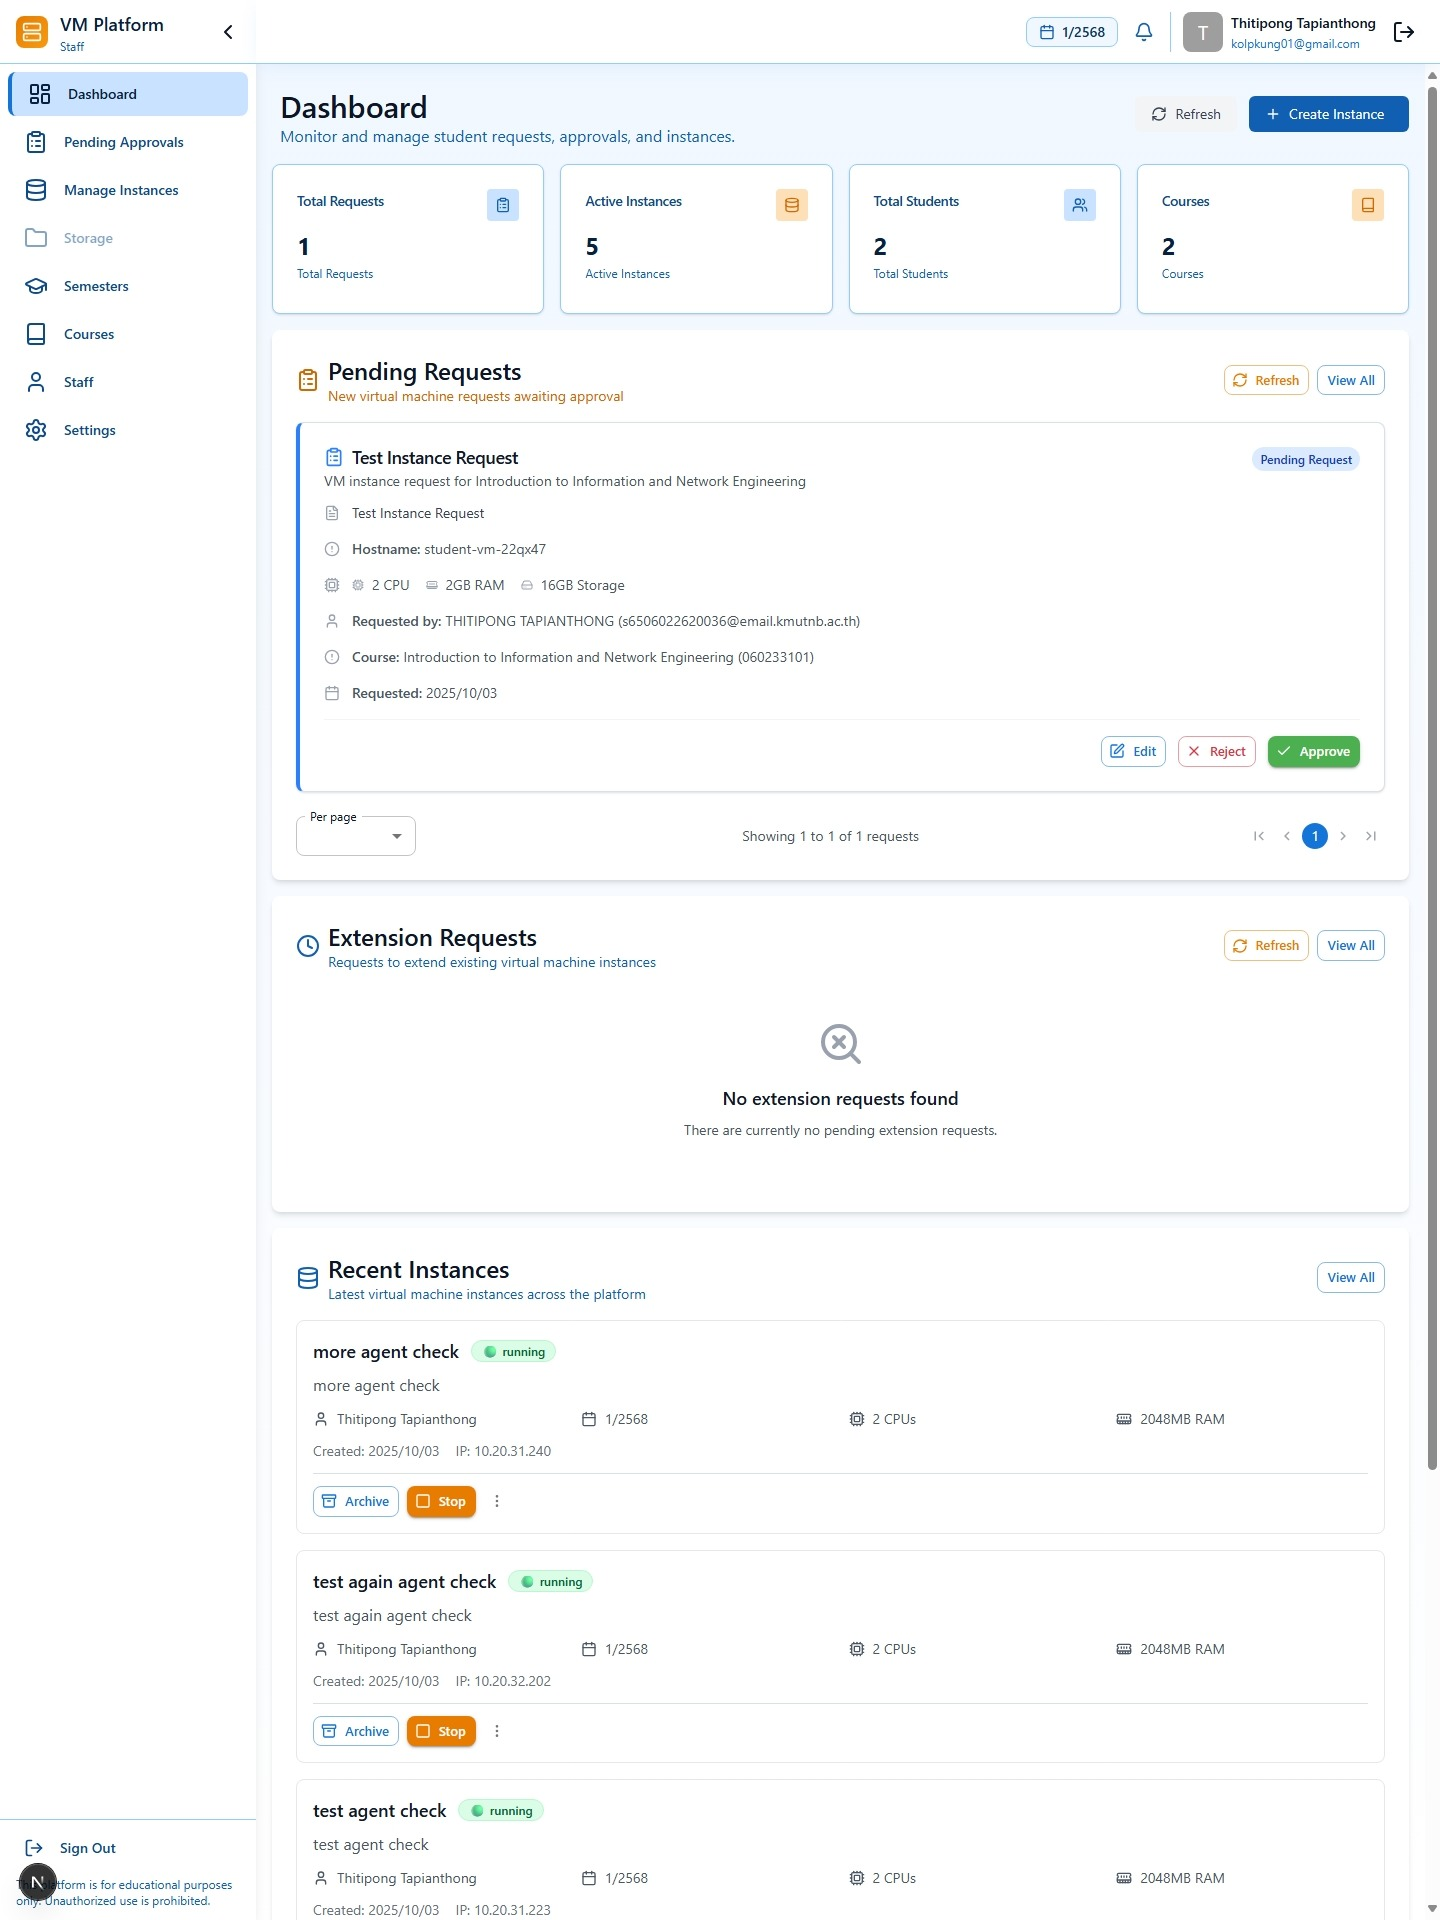
\includegraphics[width=0.9\textwidth]{Image/web/dashboard/staff/dashboard.jpeg}
}
\caption{\fontSixTeen{Dashboard หลักสำหรับอาจารย์และเจ้าหน้าที่}}
\label{fig4:StaffDashboard}
\end{figure}

\hspace*{1.5em}
อาจารย์และเจ้าหน้าที่สามารถจัดการหลักสูตรและเทอมการศึกษา ดังแสดงในภาพที่ \ref{fig4:CourseManagement} ซึ่งช่วยให้สามารถกำหนดทรัพยากรและสิทธิ์การเข้าถึงสำหรับแต่ละวิชาได้อย่างเหมาะสม

\begin{figure}[htbp]
\centering
\adjustbox{frame, width=0.9\textwidth}{
    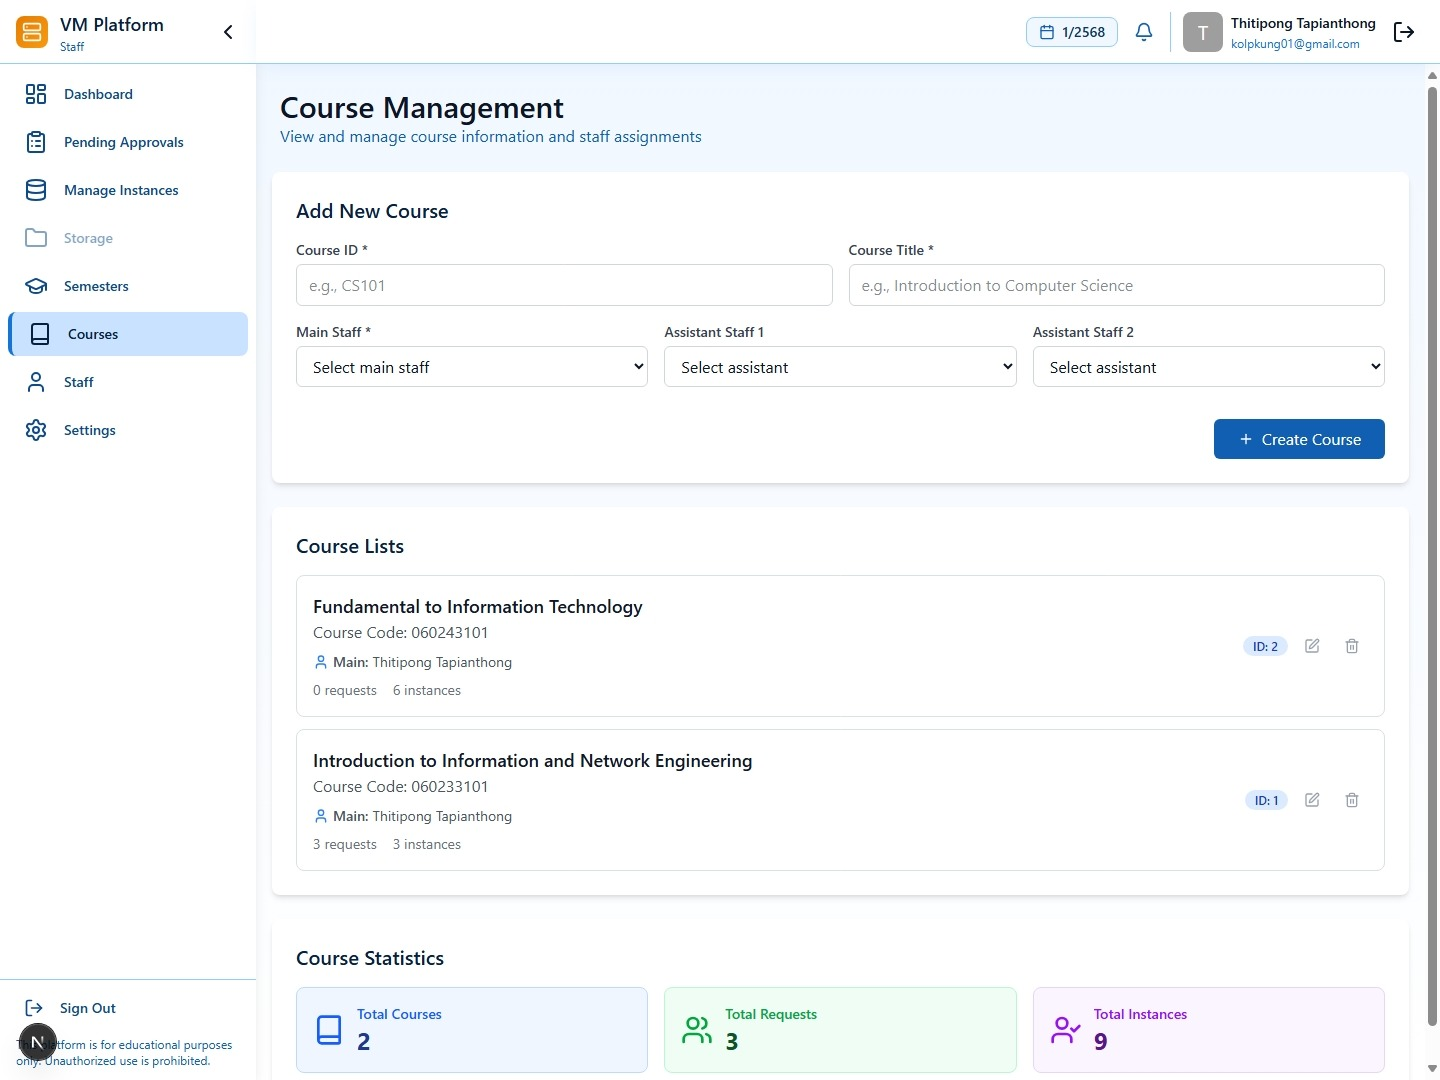
\includegraphics[width=0.9\textwidth]{Image/web/dashboard/staff/courses.jpeg}
}
\caption{\fontSixTeen{หน้าจัดการหลักสูตรและรายวิชา}}
\label{fig4:CourseManagement}
\end{figure}

\hspace*{1.5em}
นอกจากนี้ ระบบยังมีหน้าสำหรับการอนุมัติคำขอต่าง ๆ จากนักศึกษา ดังแสดงในภาพที่ \ref{fig4:PendingApproval} ซึ่งช่วยให้อาจารย์สามารถตรวจสอบและอนุมัติคำขอได้อย่างมีประสิทธิภาพ

\begin{figure}[htbp]
\centering
\adjustbox{frame, width=0.9\textwidth}{
    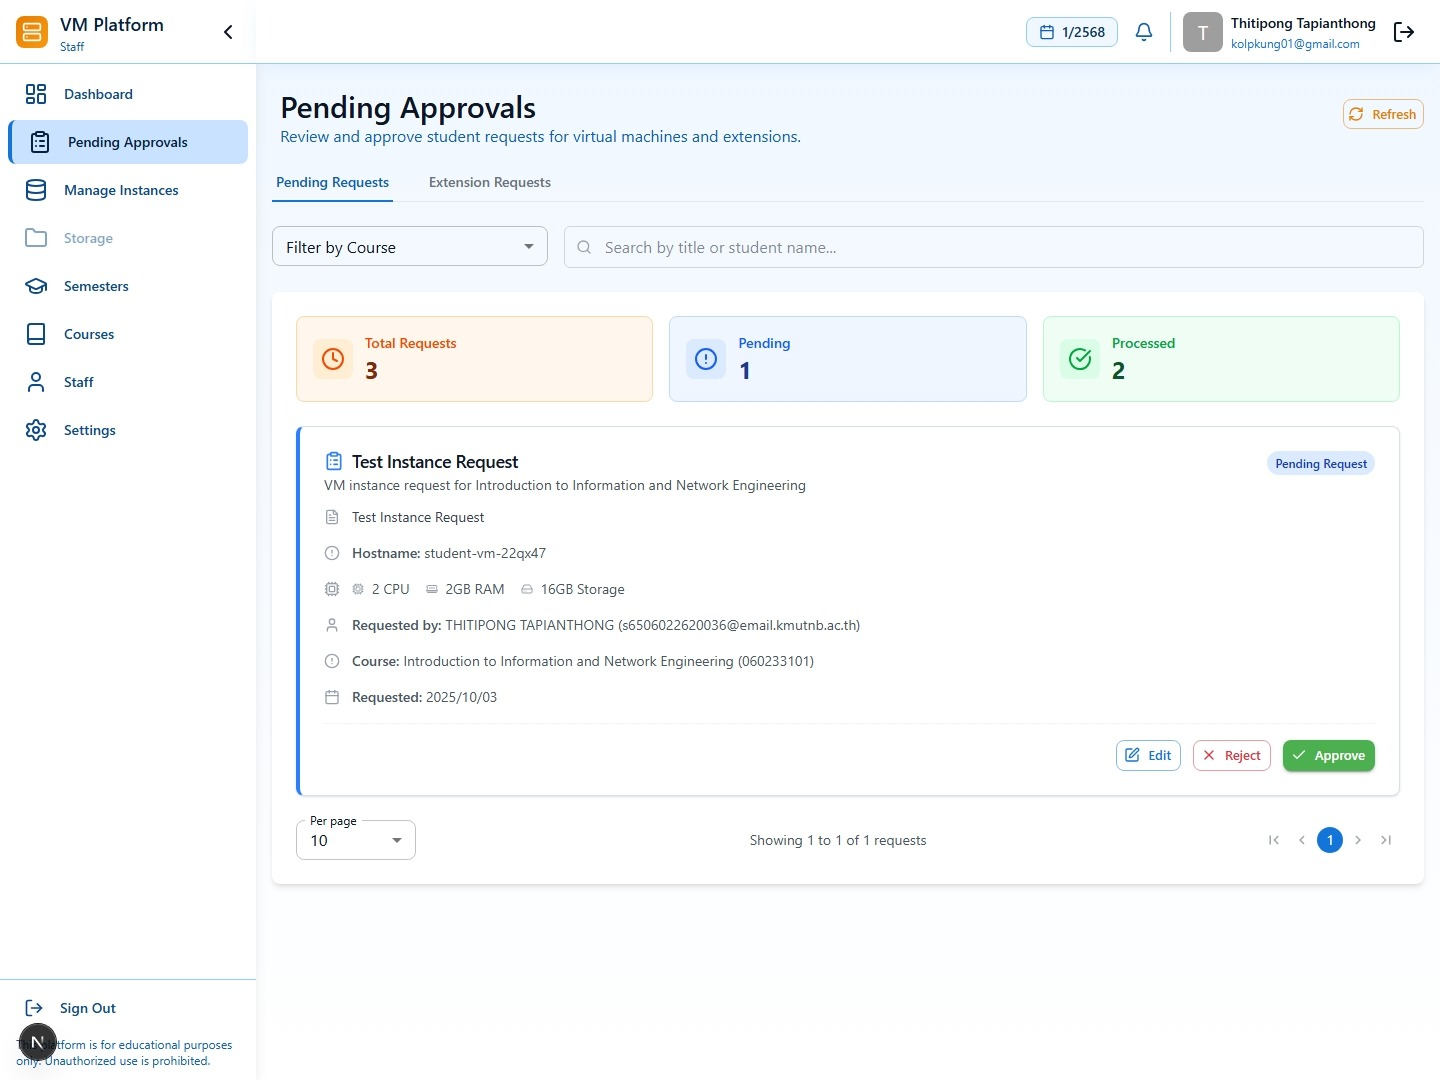
\includegraphics[width=0.9\textwidth]{Image/web/dashboard/staff/pending_approval.jpeg}
}
\caption{\fontSixTeen{หน้าอนุมัติคำขอที่รอดำเนินการ}}
\label{fig4:PendingApproval}
\end{figure}

\subsection{ระบบจัดการแบบ Role-Based Access Control}
\hspace*{1.5em}
ระบบได้นำเอา Role-Based Access Control (RBAC) มาใช้ในการจัดการสิทธิ์การเข้าถึงข้อมูลและฟังก์ชันต่าง ๆ โดยแบ่งผู้ใช้เป็น 3 กลุ่มหลัก คือ นักศึกษา อาจารย์ และผู้ดูแลระบบ ซึ่งแต่ละกลุ่มจะมีสิทธิ์และหน้าที่ที่แตกต่างกันตามความเหมาะสม

\hspace*{1.5em}
การออกแบบระบบในลักษณะนี้ช่วยให้การจัดการความปลอดภัยของข้อมูลเป็นไปอย่างมีประสิทธิภาพ และผู้ใช้แต่ละกลุ่มจะเห็นเฉพาะข้อมูลและฟังก์ชันที่เกี่ยวข้องกับหน้าที่ของตนเอง ทำให้การใช้งานง่ายขึ้นและลดความเสี่ยงในการเข้าถึงข้อมูลที่ไม่เหมาะสม